% What the Kronecker restriction *is*, drawn instead of indexed.
%
% Replaces the sentence in Section 3 that defined the admissible family as
% Gr(k1,n1) x Gr(k2,n2) embedded in Gr(k1k2, n1n2). Both bases occupy the same
% slot -- a rank-k basis for a vectorised two-axis measurement -- so the only
% thing a reader must see is the structure inside it: on the left every entry is
% free, on the right the matrix is a block grid whose every block is the SAME
% U_1 motif rescaled by one entry of U_2.
%
% Illustrative dimensions n1=3, n2=2, k1=k2=2, so the vec dimension is 6 and
% k=4. Cell counts show axis structure, not the experiment's real sizes
% (C=8, T=256, k_c=2, k_t=3).
%
% Geometry: one physical edge length per symbolic axis, reused everywhere; the
% two bases share an identical 6x4 face because they share a slot; the four
% Kronecker blocks tile their parent exactly; U_1 is 3x2 and U_2 is 2x2, drawn
% at those aspects.
%
% Build:  latexmk -pdf classes.tex
\documentclass[border=3pt]{standalone}
\usepackage{tikz}
\usepackage{amsmath,amssymb}

% Okabe-Ito, matching Figure 1 so each role keeps one colour across the paper.
\definecolor{roleA}{HTML}{0072B2}   % first-axis factor  U_1
\definecolor{roleB}{HTML}{E69F00}   % second-axis factor U_2
\definecolor{neutral}{HTML}{85898F} % unrestricted: no structure to name

% Every coordinate component is braced; TikZ will not parse `*` in a bare
% coordinate expression.
\newcommand{\cell}[4]{\fill[#4, rounded corners=0.35pt]
  ({#1+0.07},{#2+0.07}) rectangle ({#1+#3-0.07},{#2+#3-0.07});}

% Thin neutral brackets around a face of width #1 and height #2 (in mm).
\newcommand{\brackets}[2]{%
  \draw[black!60, line width=0.45pt] (-1.0,-1.0) -- (-1.0,{#2+1.0});
  \draw[black!60, line width=0.45pt] (-1.0,-1.0) -- (0.7,-1.0);
  \draw[black!60, line width=0.45pt] (-1.0,{#2+1.0}) -- (0.7,{#2+1.0});
  \draw[black!60, line width=0.45pt] ({#1+1.0},-1.0) -- ({#1+1.0},{#2+1.0});
  \draw[black!60, line width=0.45pt] ({#1+1.0},-1.0) -- ({#1-0.7},-1.0);
  \draw[black!60, line width=0.45pt] ({#1+1.0},{#2+1.0}) -- ({#1-0.7},{#2+1.0});}

\begin{document}
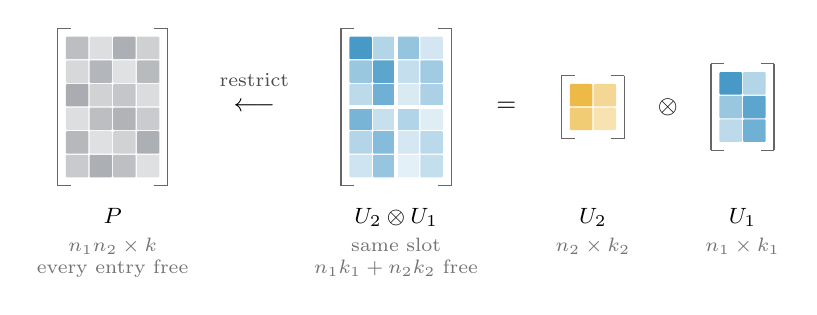
\begin{tikzpicture}[x=1mm, y=1mm, font=\footnotesize]

\def\s{3.0}        % one matrix cell, reused for every axis everywhere
\def\gapA{24}      % gutter: unrestricted -> separable
\def\gapB{16}      % gutter: separable -> factors

\pgfmathsetmacro{\wBasis}{4*\s}    % k = k1 k2 = 4
\pgfmathsetmacro{\hBasis}{6*\s}    % n1 n2 = 6
\pgfmathsetmacro{\xB}{\wBasis+\gapA}
\pgfmathsetmacro{\xC}{\xB+\wBasis+\gapB}

% ------------------------------------------------------- (a) unrestricted
% Illustrative lightness, deliberately non-periodic: there is no motif to see.
\begin{scope}
  \foreach \rw/\cl/\sh in {
    0/0/55, 0/1/28, 0/2/68, 0/3/40,  1/0/33, 1/1/62, 1/2/25, 1/3/58,
    2/0/70, 2/1/38, 2/2/48, 2/3/30,  3/0/28, 3/1/55, 3/2/64, 3/3/44,
    4/0/60, 4/1/26, 4/2/38, 4/3/68,  5/0/45, 5/1/68, 5/2/54, 5/3/26}
    {\cell{\cl*\s}{(5-\rw)*\s}{\s}{neutral!\sh}}
  \brackets{\wBasis}{\hBasis}
  \node[anchor=north] at ({\wBasis/2}, -2.6) {$P$};
  \node[anchor=north, font=\scriptsize, text=black!55, align=center]
    at ({\wBasis/2}, -6.4) {$n_1n_2\times k$\\every entry free};
\end{scope}

% ------------------------------------------------------- (b) separable
% Same face, now a 2x2 grid of 3x2 blocks; block (j,l) is U_2[j,l] times U_1.
% Lightness carries that product, so the repeated motif is what the eye sees.
\begin{scope}[shift={(\xB,0)}]
  \foreach \bjj/\bll/\wt in {0/0/1.00, 0/1/0.58, 1/0/0.74, 1/1/0.42}{
    \foreach \ii/\mm/\lv in {0/0/72, 0/1/30, 1/0/40, 1/1/64, 2/0/26, 2/1/56}{
      \pgfmathsetmacro{\shade}{\lv*\wt}
      \pgfmathsetmacro{\xx}{(\bll*2+\mm)*\s}
      \pgfmathsetmacro{\yy}{(5-(\bjj*3+\ii))*\s}
      \cell{\xx}{\yy}{\s}{roleA!\shade}
    }
  }
  % Block gutters: wide white lines, so the tiling reads as structure not texture.
  \draw[white, line width=1.5pt] (0,{3*\s}) -- ({\wBasis},{3*\s});
  \draw[white, line width=1.5pt] ({2*\s},0) -- ({2*\s},{\hBasis});
  \brackets{\wBasis}{\hBasis}
  \node[anchor=north] at ({\wBasis/2}, -2.6) {$U_2\otimes U_1$};
  \node[anchor=north, font=\scriptsize, text=black!55, align=center]
    at ({\wBasis/2}, -6.4) {same slot\\$n_1k_1+n_2k_2$ free};
\end{scope}

% ------------------------------------------------------- the two factors
% Faces are vertically centred on the basis; their labels are placed outside
% the scopes so all four symbol/shape rows share one baseline.
\pgfmathsetmacro{\xD}{\xC+2*\s+13}
\begin{scope}[shift={(\xC,{2*\s})}]
  \foreach \jj/\ll/\lv in {0/0/72, 0/1/42, 1/0/54, 1/1/30}
    {\cell{\ll*\s}{(1-\jj)*\s}{\s}{roleB!\lv}}
  \brackets{2*\s}{2*\s}
\end{scope}
\begin{scope}[shift={(\xD,{1.5*\s})}]
  \foreach \ii/\mm/\lv in {0/0/72, 0/1/30, 1/0/40, 1/1/64, 2/0/26, 2/1/56}
    {\cell{\mm*\s}{(2-\ii)*\s}{\s}{roleA!\lv}}
  \brackets{2*\s}{3*\s}
\end{scope}
\node[anchor=north] at ({\xC+1*\s}, -2.6) {$U_2$};
\node[anchor=north, font=\scriptsize, text=black!55]
  at ({\xC+1*\s}, -6.4) {$n_2\times k_2$};
\node[anchor=north] at ({\xD+1*\s}, -2.6) {$U_1$};
\node[anchor=north, font=\scriptsize, text=black!55]
  at ({\xD+1*\s}, -6.4) {$n_1\times k_1$};

% ---------------------------------------------------------- operators
\node[font=\small] at ({\wBasis+\gapA/2}, {\hBasis/2}) {$\longleftarrow$};
\node[anchor=south, font=\scriptsize, text=black!70]
  at ({\wBasis+\gapA/2}, {\hBasis/2+1.4}) {restrict};
\node[font=\small] at ({\xB+\wBasis+\gapB/2}, {\hBasis/2}) {$=$};
\node[font=\small] at ({\xD-6.5}, {\hBasis/2}) {$\otimes$};

\end{tikzpicture}
\end{document}
